\chapter{The Latte Framework}

\section{Introduction}
The Latte framework forms the basis for almost all of the reconstruction algorithms described in this thesis. It acts as both a set of utilities and a unifying central control mechanism. This chapter discusses several of the algorithms provided, ending with an overview of the control structures of the Latte framework itself. Some components of Latte form a significant contribution to the work in this thesis, and are discussed separately in subsequent chapters.

\section{Nearest Neighbour Search using \acs{KDTree}}\label{sec:latte_kdtree}
The \ac{KDTree} is a data structure for partitioning a $k$-dimensional space by representing the points as nodes in a binary tree. Using a \ac{KDTree} it is possible to perform nearest-neighbour search in $O(\log N)$ time\citep{Bentley1975} (though the tree itself is built in $O(kN\log N)$ time), compared with the brute-force search complexity of $O(N^2)$. An introductory tutorial on \aclp{KDTree} appears in \citep{Moore1991}. The \ac{KDTree} is not a clustering algorithm, but its rapid near-neighbour search forms a central part of several clustering algorithms, as well as being used for the charge weighting (see chapter \ref{sec:cellularautomaton_charge_weighting}) and cell generation (\ref{sec:cellularautomaton_cell_generation}) stages of the \acl{CA} track reconstruction procedure.

The implementation currently used is that of the \emph{SciPy}\citep{SciPy} library of Python code for scientific computing.

\section{Charge Weighting}\label{sec:cellularautomaton_charge_weighting}
Data from a \ac{LAr TPC} is assumed to be in the form of $(x, y, z)$ voxels with an associated charge deposit $Q$. The voxel shape is determined entirely by the readout mechanism; a 2D readout plane determines the $xy$ resolution while the readout frequency determines the $z$ resolution as expected for a \ac{TPC}. This structure is retained in the Geant4 simulation through the use of cubic voxels with a side length of $1\mm$. In order to transform this data into a representation more closely resembling the true passage of ionising radiation through the detector, a charge weighting procedure is applied. This procedure adjusts the spatial coordinates of each charge deposit (voxel) by taking the charge-weighted average of the spatial coordinates of all hits within a sphere of some radius (default: $2\mm$) centered on that voxel:

\begin{equation}\label{eqn:charge_weighted_avg_position}
	\vec{x}^\prime = \frac{\displaystyle \sum_i \vec{x}_i Q_i}{\displaystyle \sum_i Q_i}
\end{equation}

The neighbouring hits are discovered using the \ac{KDTree} algorithm described in section \ref{sec:latte_kdtree}.

Charge weighting in this way moves the position of each charge deposit closer to the local charge cloud, bringing track-like charge deposits closer to a straight line (see figure \ref{fig:ca_charge_weighting}). In each case the unweighted positions of neighbours are used to compute the weighted position of a central charge deposit, resulting in a stable, deterministic output.

\begin{figure}
\centering
\subfigure[Hits as central points of voxels]{
	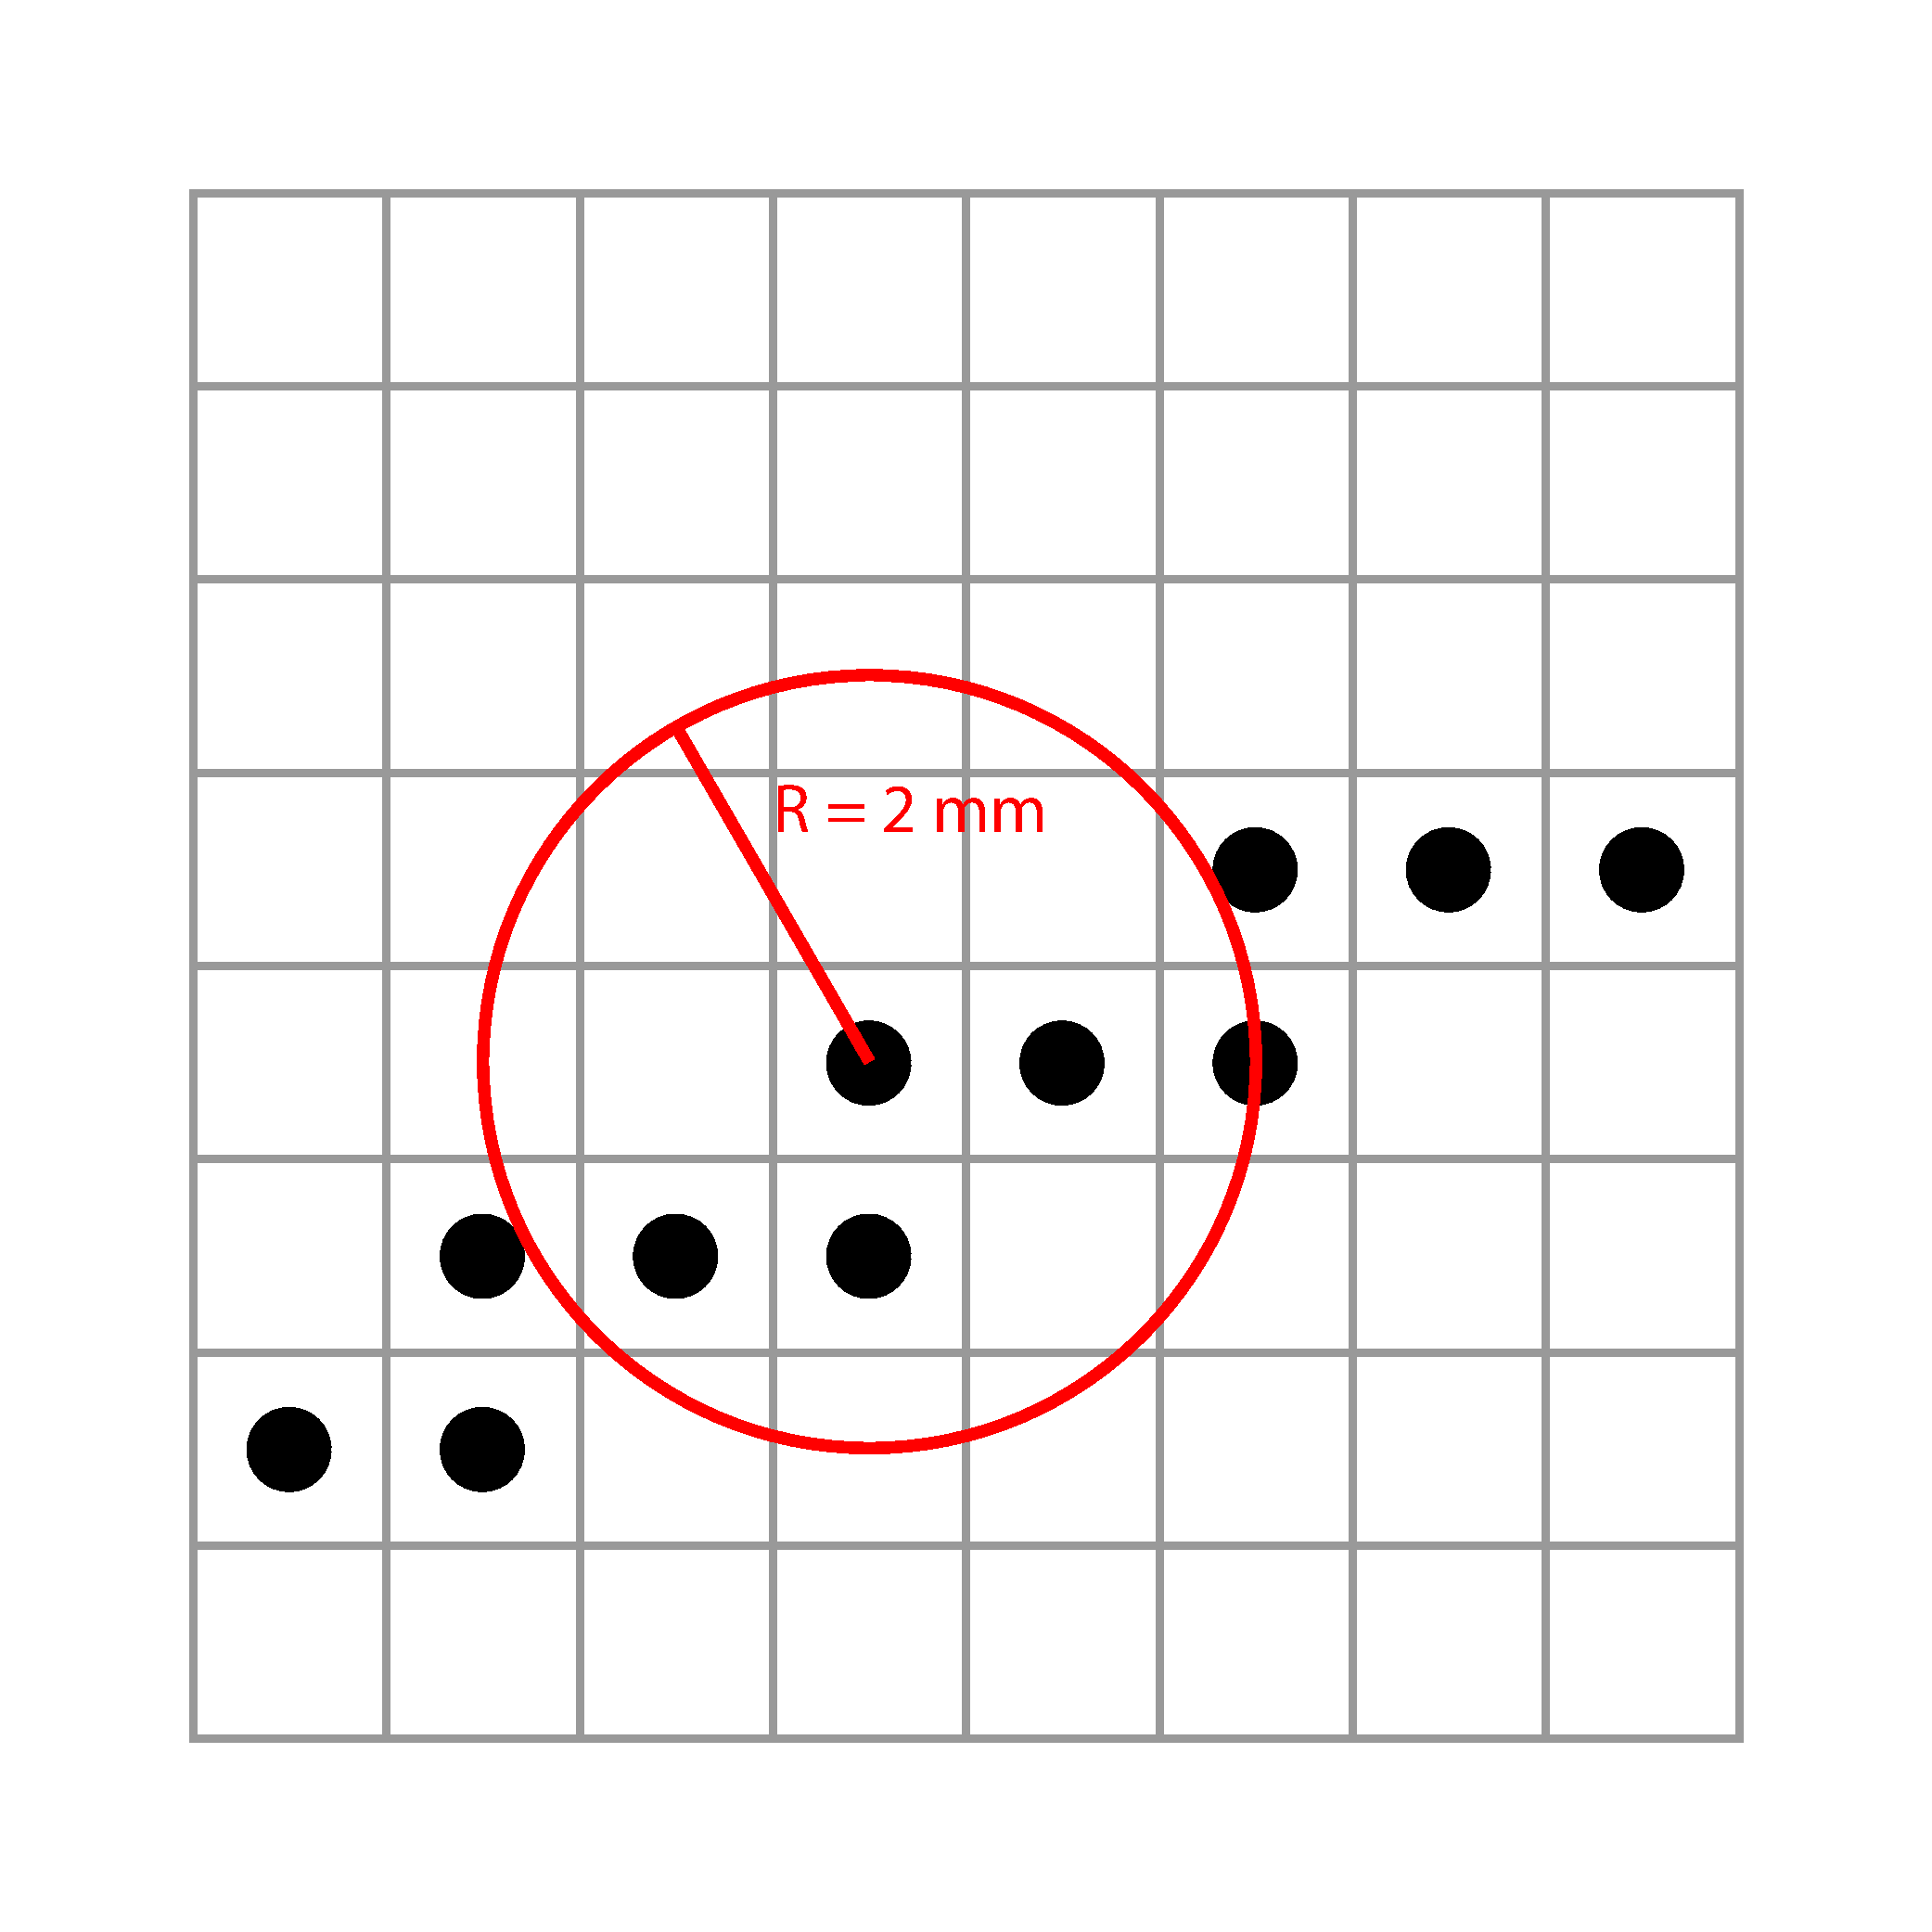
\includegraphics[width=0.4\textwidth]{chapters/cellularautomaton_images/ChargeWeighting1}
	\label{fig:ca_charge_weighting_1}
}
\subfigure[Hits shifted from voxel centres]{
	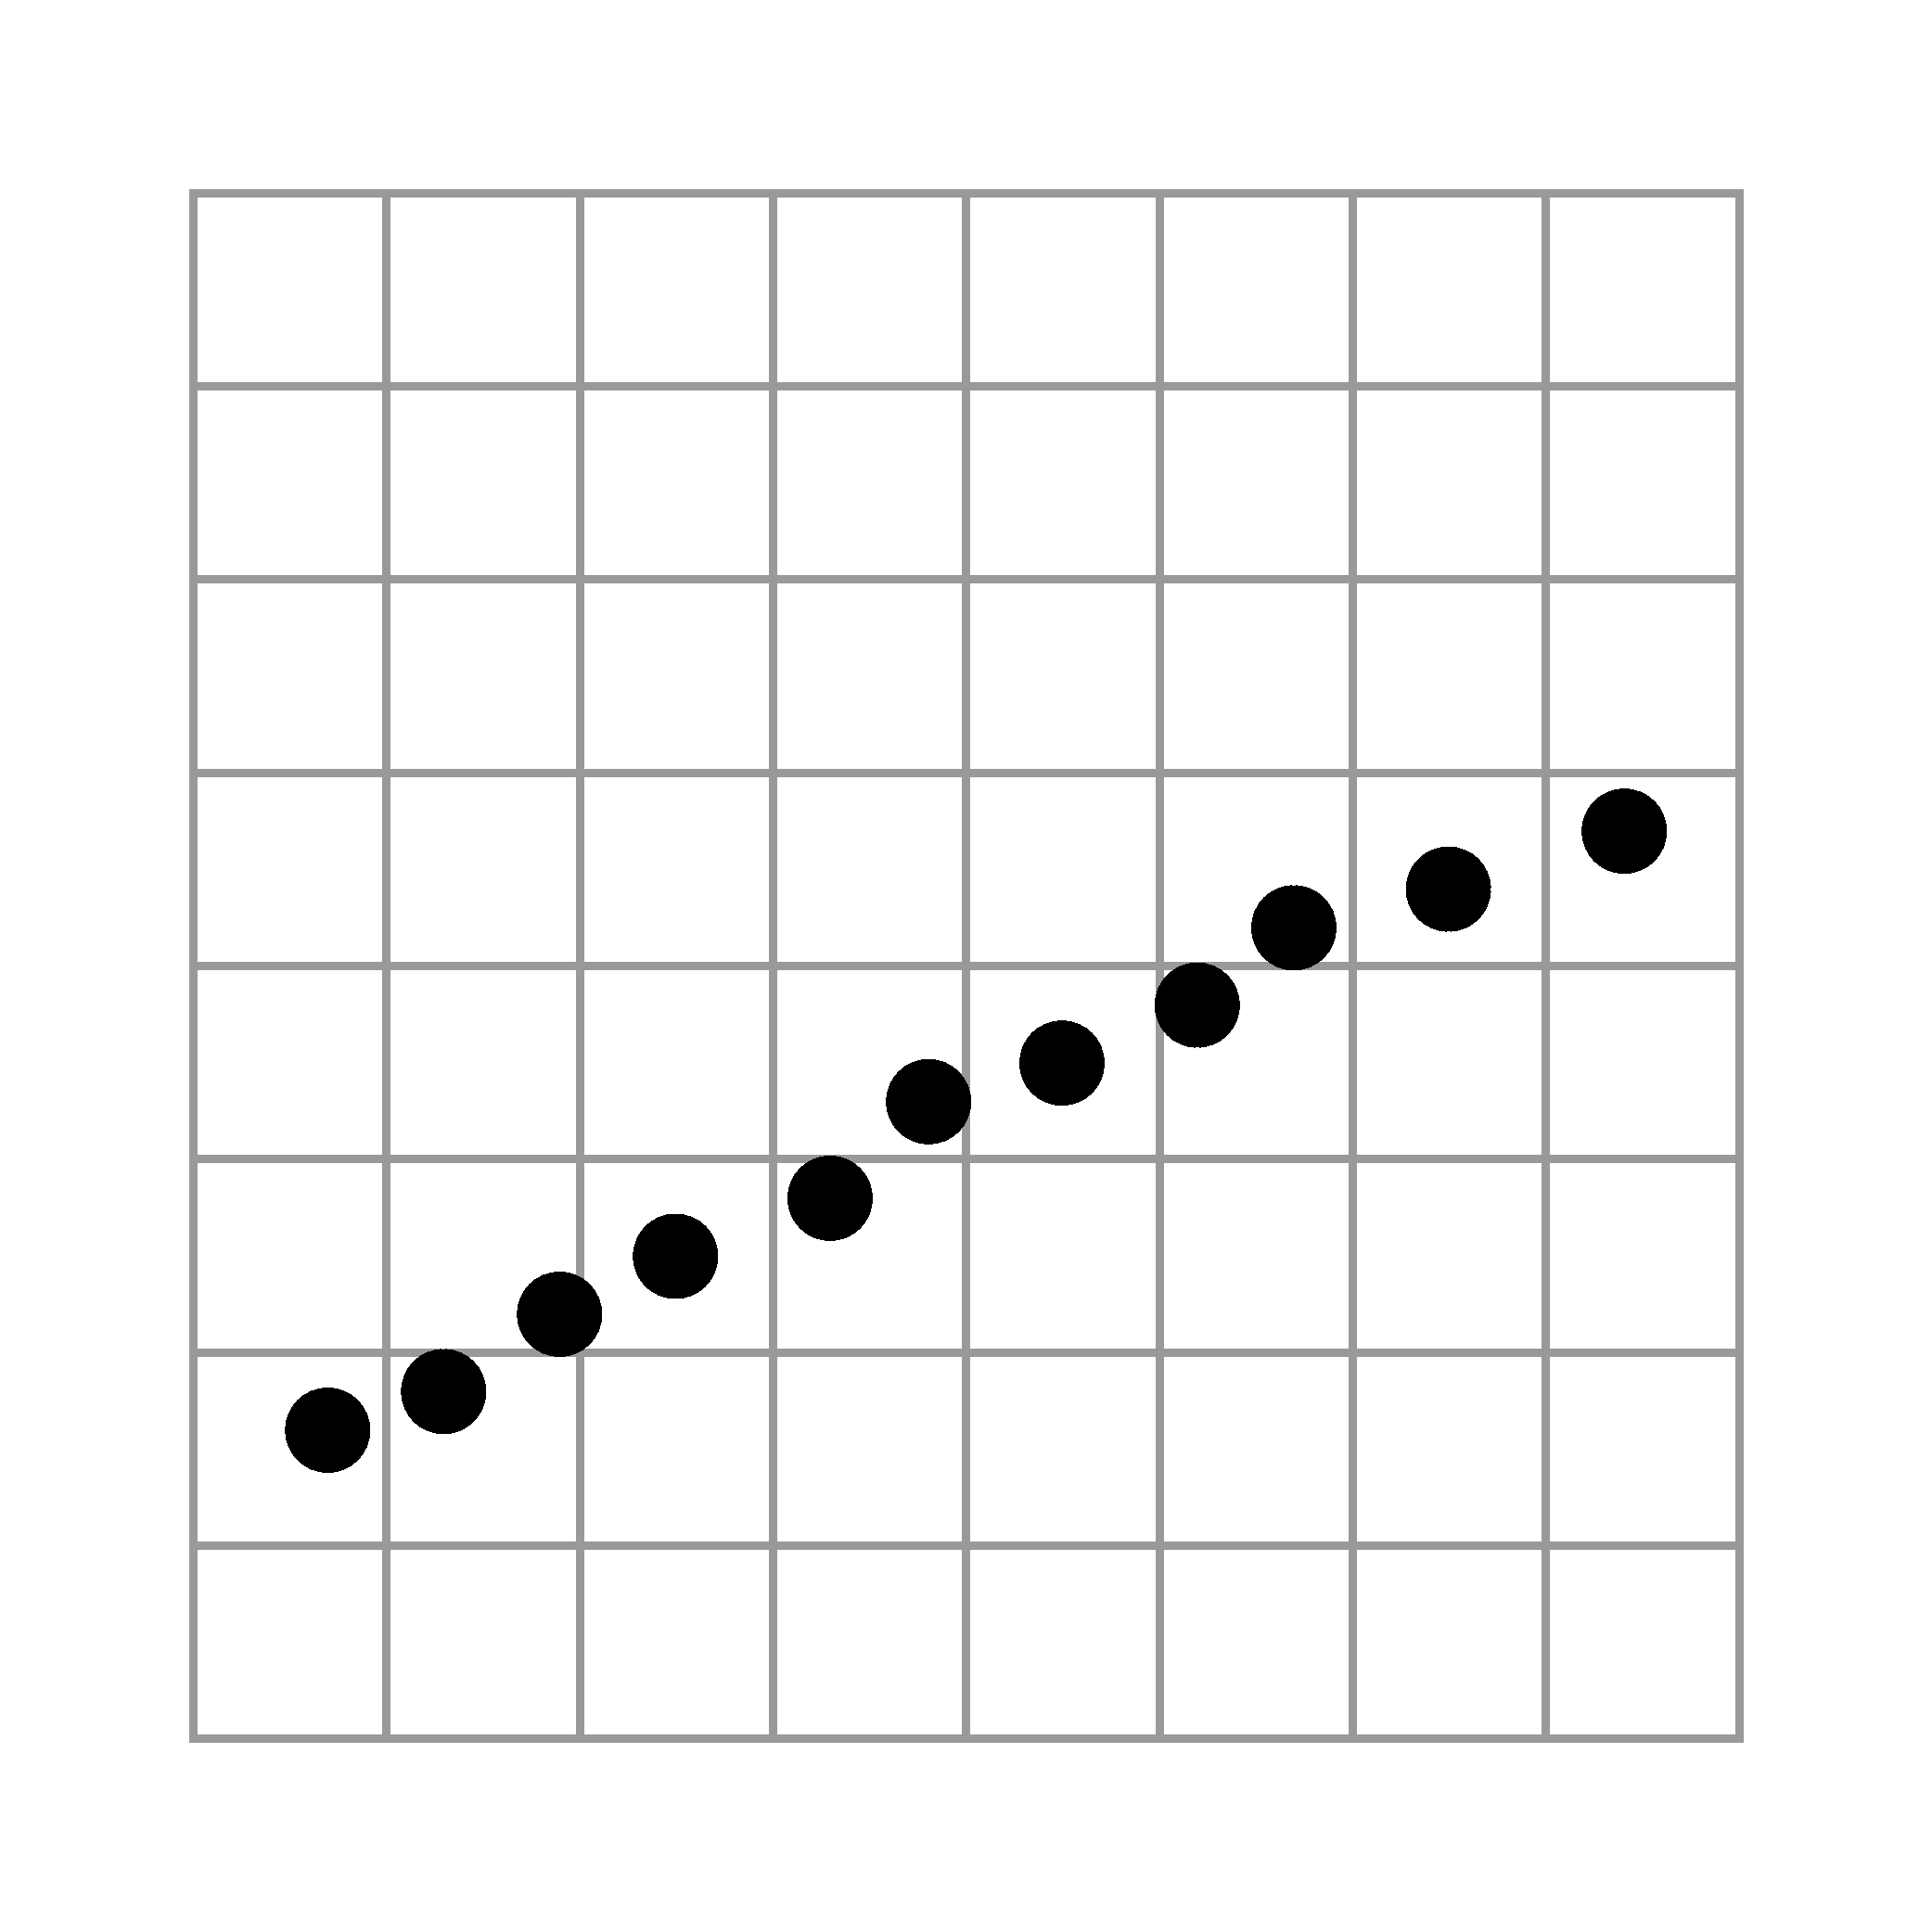
\includegraphics[width=0.4\textwidth]{chapters/cellularautomaton_images/ChargeWeighting2}
	\label{fig:ca_charge_weighting_2}
}
\caption[Diagram of the effect of charge weighting on hit position]{\label{fig:ca_charge_weighting}Schematic diagram of the effect of the charge weighting procedure on hit positions. In \subref{fig:ca_charge_weighting_1} each hit is positioned at the centre of a voxel. In \subref{fig:ca_charge_weighting_2} the hit positions have been adjusted based on the charge-weighted positions of surrounding hits within a $2\mm$ radius; this shifts them from the voxel centres and out of a regular grid structure.}
\end{figure}

\section{Density-based Clustering}
\subsection{\acs{DBSCAN}}\label{sec:latte_dbscan}
The \ac{DBSCAN} algorithm was proposed in 1996 as a means of clustering spatial data based on the varying densities of point clouds\citep{Ester1996}. The algorithm is characterised by its requirement that, for the neighbourhood $\epsilon$ around a given point in the cluster, the number of points $N$ in $\epsilon$ must exceed some threshold value $N_\mathrm{min}$. In this manner, the clustering is determined by identifying areas of high point density. Areas of low point density (i.e. any points not clustered) are identified as \emph{noise} and clustered together as such.

The \ac{DBSCAN} algorithm has been applied to spatial data obtained from a \ac{LAr TPC} by the ArgoNeuT experiment\cite{Spitz2011} to identify clusters in two 2D views, which are subsequently recombined into 3D based on wire readout timing information.

\ac{DBSCAN} has two configurable parameters, $\epsilon$, the radius around a given point within which neighbours must lie, and $N_\mathrm{min}$, the minimum number of those neighbours for a point to be considered part of a dense cluster. While these parameters can be optimised, they remain global, and \ac{DBSCAN} will not typically identify regions of changing density and cluster accordingly. This tends to result in a \ac{DBSCAN} clustering which wraps around the vertex of charged-current neutrino events.

\subsection{\acs{OPTICS}}
The \ac{OPTICS} algorithm\citep{Ankerst1999} extends \ac{DBSCAN} by performing a \emph{hierarchical clustering}; an ordering operation which is equivalent to giving the density-based clusterings associated with a broad range of values of the parameter $\epsilon$. For example, given a fixed value of $N_\mathrm{min}$, clusters obtained with a small $\epsilon$ (that is, high density clusters) are completely contained within the clusters obtained for a larger $\epsilon$ (lower density). \ac{OPTICS} exploits this relationship to provide information about the clustering on all $\epsilon$ scales, allowing clusters to be extracted from spatial data with varying densities.

\section{Feature Detection}\label{sec:latte_feature_detection}
Feature detection refers to the procedure of locating interest points within an image or event. Latte provides two-dimensional feature detection using the method described in \citep{Morgan2010}. 

\section{Feature Masking}
Latte provides a service to \emph{mask out} (remove) hits within a spherical region around a feature. The feature masking service presents a new view of the data, which does not include hits positioned less than some radius away from a central point. Each such point can be the location of a feature as determined by the feature detection algorithms of section \ref{sec:latte_feature_detection}, or in a special case the point $(0,0,0)$, referred to as \emph{origin masking}.

This service is useful because it allows algorithms to run on modified views of the event data, which often produces better results. One example would be in a clustering algorithm such as DBSCAN (see \ref{sec:latte_dbscan}), where the local point density affects the clustering. Introducing a gap which corresponds to some feature such as a vertex results in a better clustering of tracks.

\section{Track Merging}
%TODO: Write this!

\section{Truth Information}
%TODO: Write this!

\section{Range Cuts}
%TODO: Write this!

\section{Latte Control}
Latte Control is a mechanism for applying a sequence of algorithms to a set of events. In its simplest form, it allows the user to set up a \emph{pipeline} composed of service algorithms which are run in sequence on each event stored in a {\sc Root} file.

\subsection{Services \& Event Wrappers}
Algorithms made available in the Latte framework can be used with Latte Control in one of two ways. For general purpose reconstruction algorithms, Latte Control provides a corresponding \emph{Service}, which accepts an event object and performs some task. For example, the \emph{Merging} service provides an interface to the track merging algorithms provided in Latte and, when called, runs them on the active track selection. Services usually provide algorithms which are processor-intensive and add new information to the event, for example the allocation of hits to clusters, or the merging of multiple clusters based on certain criteria. Services typically augment an event with the additional information they are able to provide.

In contrast, there are many cases where the goal of an algorithm is to present a different \emph{view} of the same data. One such example is the charge weighting algorithm, which shifts the position of each hit. Such algorithms are typically brought into the Latte Control framework as \emph{event wrappers}, which intercept attempts to access certain data which are already associated with an event, and present some modified version of that data. In this way, the original data is preserved, and can be retrieved by simply \emph{unwrapping} the event. Each event wrapper provides a \emph{wrapping service} which is used to apply the wrapper at some arbitrary point.

\subsection{Pipelines}
Each event is processed by a \emph{pipeline}, which is simply a sequence of service objects that are called in turn. Some services perform complex tasks such as clustering, while others wrap or unwrap an event, thus changing the views of data available for subsequent services. As events propagate through the pipeline, reconstructed information is added to them by the appropriate services, and may be written to disk (for example) at various points.

Since a Pipeline appears (to an outside observer) as just another callable object which accepts events, it is possible to put pipelines within pipelines, for example to group related services into logical \emph{tasks} (such as grouping clustering and merging of tracks into a \emph{tracking} task), or to provide decision making, using a service which chooses to execute one of several pipelines based on the value (or existence) of certain data in the event.

This flexibility means that the pipeline structure of Latte Control is capable of performing complicated analyses without needing further core support. A user can simply stick together the components they need, in the correct order, then leverage the power of Latte Control to run their analysis job over the available data.

\subsection{Event Loops}
At the highest level, Latte Control provides an event loop which is capable of reading a range of events from a {\sc Root} file and passing each event in turn through a pipeline of Latte Control services. In this manner, it is possible to easily write reconstruction scripts which configure a number of services, stick them together in an arbitrary order into a pipeline, and have that pipeline applied to each event in a file. This provides a powerful mechanism for writing physics analysis scripts which make use of the Latte-provided services as well as intermediate or final \emph{analysis} services, using the data available in an event to measure physically useful quantities. Since the objects representing pipeline segments persist between events, they can also be used to build up statistics over an entire set of events. When the event loop finishes, the analysis object can be queried for the set of statistical data it has collected.

